% ============================================================================
%  Profiling section  —  drop into a two-column A4 article.
%  Requires in the preamble:   \usepackage{graphicx,booktabs}
%  and (if this .tex is at the repo root):
%      \graphicspath{{visual/plots/}}
%  Otherwise edit the \includegraphics paths below.
%  Wide landscape plots use figure* (span both columns); the narrower ones
%  use a single-column figure. The Gantt timelines are intentionally omitted.
% ============================================================================
\section{Profiling}
\label{sec:profiling}

We profile an 8B-parameter LLaMA-style model (32 layers, hidden 4096,
FFN 14336, 32/8 query/KV heads, sequence length 4096, global batch 256,
micro-batch 2) trained on 32 GH200 GPUs (8 nodes $\times$ 4). The
parallel layout is tensor-parallel $\mathrm{TP}=2$, pipeline-parallel
$\mathrm{PP}=2$ and data-parallel $\mathrm{DP}=8$, with the distributed
optimizer and Megatron's \texttt{--overlap-grad-reduce} /
\texttt{--overlap-param-gather} enabled. Figure~\ref{fig:topology} shows
the resulting layout: TP groups sit intra-node on NVLink, while PP and DP
groups span nodes over the Slingshot interconnect.

We use two complementary instruments. A lightweight \emph{communication
logger} records, for every NCCL call on every rank, the collective type,
byte volume, peer set and wall/GPU duration (one JSONL file per rank);
this captures traffic volume and per-event latency. Separately, NVIDIA
Nsight Systems captures the full GPU kernel timeline over five
steady-state steps; because NCCL and compute kernels run on distinct CUDA
streams, this is what lets us measure true compute/communication overlap
(the logger cannot --- it brackets each call with CUDA events, which
synchronises and serialises it).

\subsection{Communication volume and latency (logger)}

\noindent\textbf{Per-step breakdown (Fig.~\ref{fig:perstep}).}
Mean per-rank communication time per step, stacked by event. The fused
1F1B pipeline exchange dominates the \emph{logged} time and the TP
all-reduce is a steady secondary contributor, whereas the data-parallel
collectives register almost nothing: with the distributed optimizer they
are launched asynchronously, so the logger only ever sees their
non-blocking launch. These wall times conflate transfer with waiting,
which is exactly why the overlap question needs the kernel timeline
below.

\noindent\textbf{Communication matrices (Fig.~\ref{fig:commmatrix}).}
GB sent from sender (row) to receiver (column), one panel per group type.
The structure is clean: TP traffic is confined to intra-node pairs, PP
traffic connects stage~0 to stage~1 (the 16-rank offset), and DP traffic
spreads across each 8-member group. The empty stage-1 rows in the TP and
per-layer DP panels are a logging asymmetry (those events are only logged
on stage-0 ranks), not an absence of traffic.

\noindent\textbf{Effective bandwidth (Fig.~\ref{fig:bandwidth}).}
Per-event effective bandwidth, $(\text{send}+\text{recv})/\text{wall}$.
The intra-node TP all-reduce reaches by far the highest bandwidth
(NVLink), while the inter-node PP and DP collectives are much lower
(Slingshot); blocking events are additionally depressed because their
wall time includes synchronisation wait.

\noindent\textbf{Per-rank latency (Figs.~\ref{fig:tpdplat},
\ref{fig:pairlat}) and wait heatmap (Fig.~\ref{fig:heatmap}).}
The per-rank TP/DP latencies and the per-PP-pair latencies are uniform
across ranks --- no single straggler dominates --- and the two endpoints
of each pipeline pair see matching latency, indicating the cost is
structural rather than a bad node. The heatmap of median wait per
(rank, event) makes the stage-0/stage-1 logging split visible at a
glance.

\subsection{Compute/communication overlap (Nsight)}

Figure~\ref{fig:overlap-summary} is the central result. The top panel
accounts for where every $\approx 5.5$\,s step goes: compute occupies
only 51\% of the step on stage-0 ranks (54\% on stage~1), communication
is busy for 50\% of the step but \emph{only 18\% of it is hidden behind
compute}, leaving $\sim$41\% of every step (44\% on stage~1) as
\emph{exposed} communication plus 2--8\% GPU idle. The bottom panel
attributes the exposed cost to collectives (Table~\ref{tab:exposed}).

\begin{table}[t]
  \centering
  \caption{Exposed communication per step (PP stage-0 mean) and the
    fraction of each collective hidden behind compute.}
  \label{tab:exposed}
  \begin{tabular}{lrr}
    \toprule
    Collective & Exposed (ms/step) & Hidden \\
    \midrule
    DP reduce-scatter (grad) & 965 & 10\% \\
    TP all-reduce            & 457 & 44\% \\
    PP send/recv             & 421 & 0\%  \\
    Input broadcast          & 374 & 0\%  \\
    DP all-gather (param)    & 39  & 57\% \\
    \bottomrule
  \end{tabular}
\end{table}

The dominant cost is the distributed-optimizer \textbf{gradient
reduce-scatter} ($\approx 965$\,ms, only 10\% hidden): although
\texttt{--overlap-grad-reduce} is enabled, the cross-node reduce-scatter
is bandwidth-bound on Slingshot and cannot keep up with the rate at
which gradients are produced, so on the kernel timeline it forms a solid
block at the \emph{end} of the step where no compute remains to hide it
(Fig.~\ref{fig:overlap-timeline}). TP all-reduce fares better (44\%
hidden, partly on a side stream).
Pipeline send/recv is more exposed on the last stage ($\approx 781$\,ms
vs.\ 421\,ms), reflecting the 1F1B bubble. The per-micro-batch input
broadcast appears only on stage-0 non-source ranks --- a spin-wait for
the TP-source rank's data loader (it surfaces as GPU idle on the source
ranks), i.e.\ an input-pipeline stall, not interconnect bandwidth.

\subsection{Implications for parallel layout}

Communication, not computation, gates throughput here: fully hiding it
would shrink the step from $\approx 5.5$\,s towards the $\approx 2.9$\,s
of useful compute, an $\approx 1.8\times$ speedup. Because the dominant
cost is the cross-node DP reduce-scatter, the most promising lever is to
\emph{raise TP from 2 to 4}: TP=4 stays intra-node on NVLink, halves the
per-rank gradient volume \emph{and} shrinks the DP group from 8 to 4,
attacking the reduce-scatter from both sides. We would pair this with
\texttt{--tp-comm-overlap} (to hide the larger TP all-reduce behind the
GEMMs) and a fix for the stage-0 data-loader stall, while keeping
$\mathrm{TP}\le 4$ so tensor-parallel traffic never leaves the node.

% ===== figures ============================================================

\begin{figure*}[t]
  \centering
  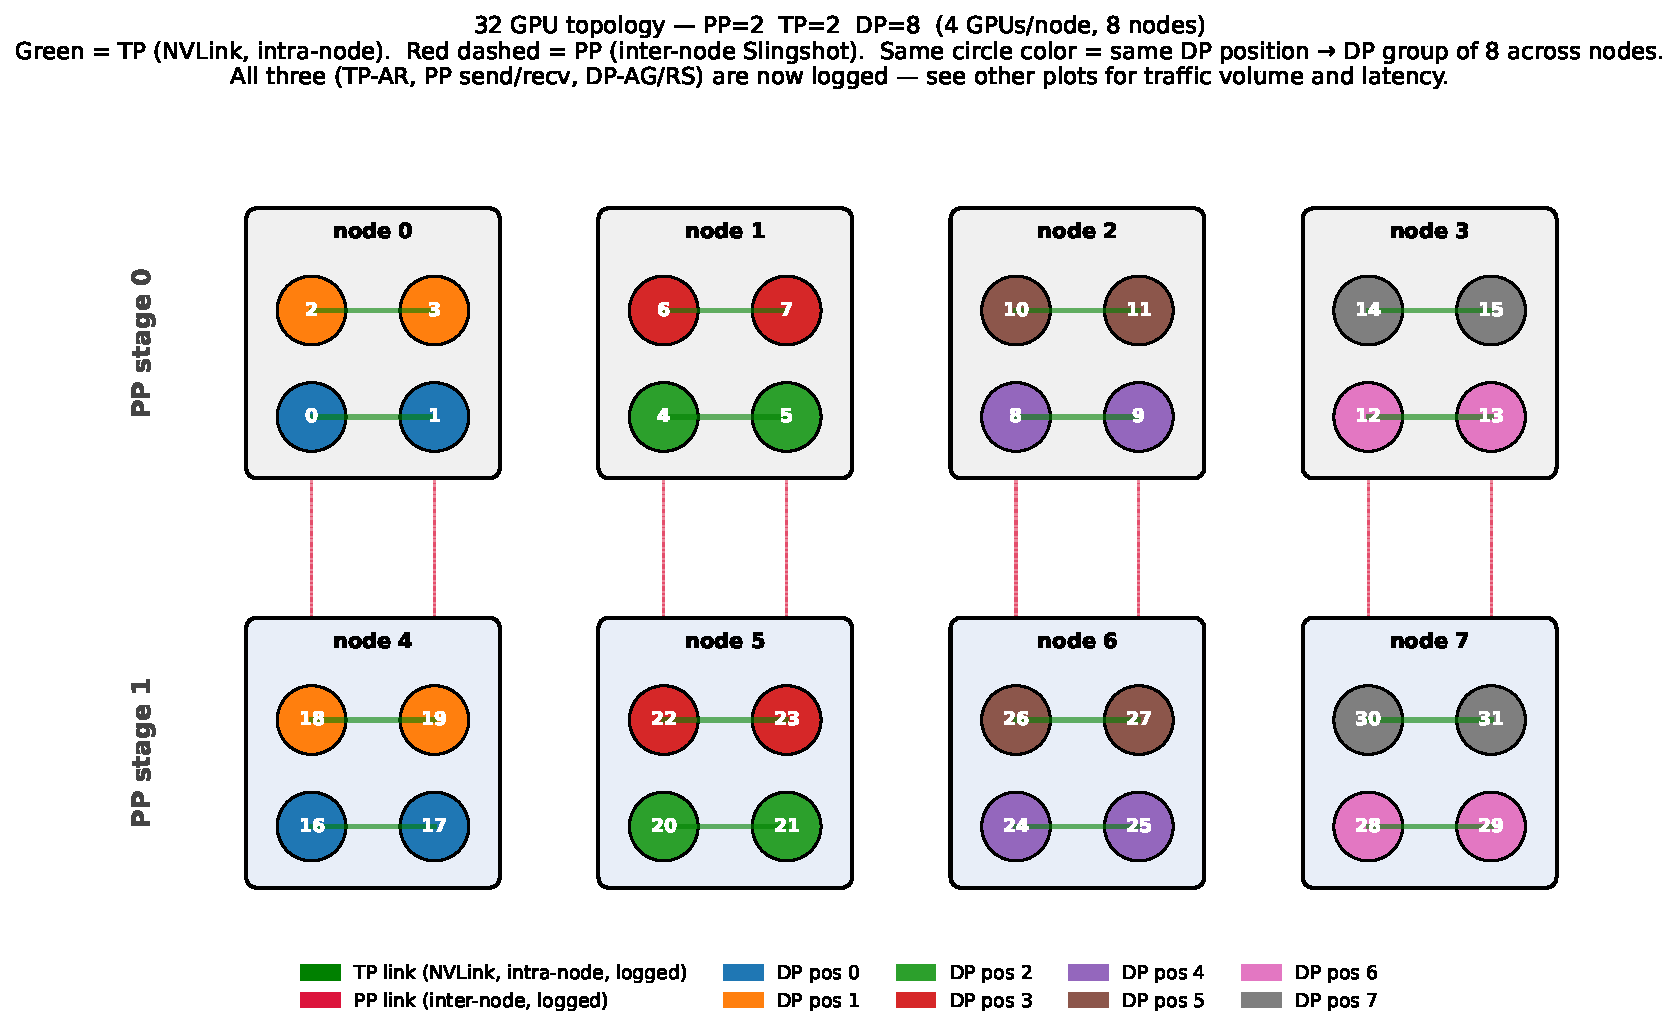
\includegraphics[width=0.9\textwidth]{topology.pdf}
  \caption{The 32-GPU layout: TP=2 (NVLink, intra-node), PP=2 (stages
    across nodes), DP=8 (same colour = same DP position).}
  \label{fig:topology}
\end{figure*}

\begin{figure*}[t]
  \centering
  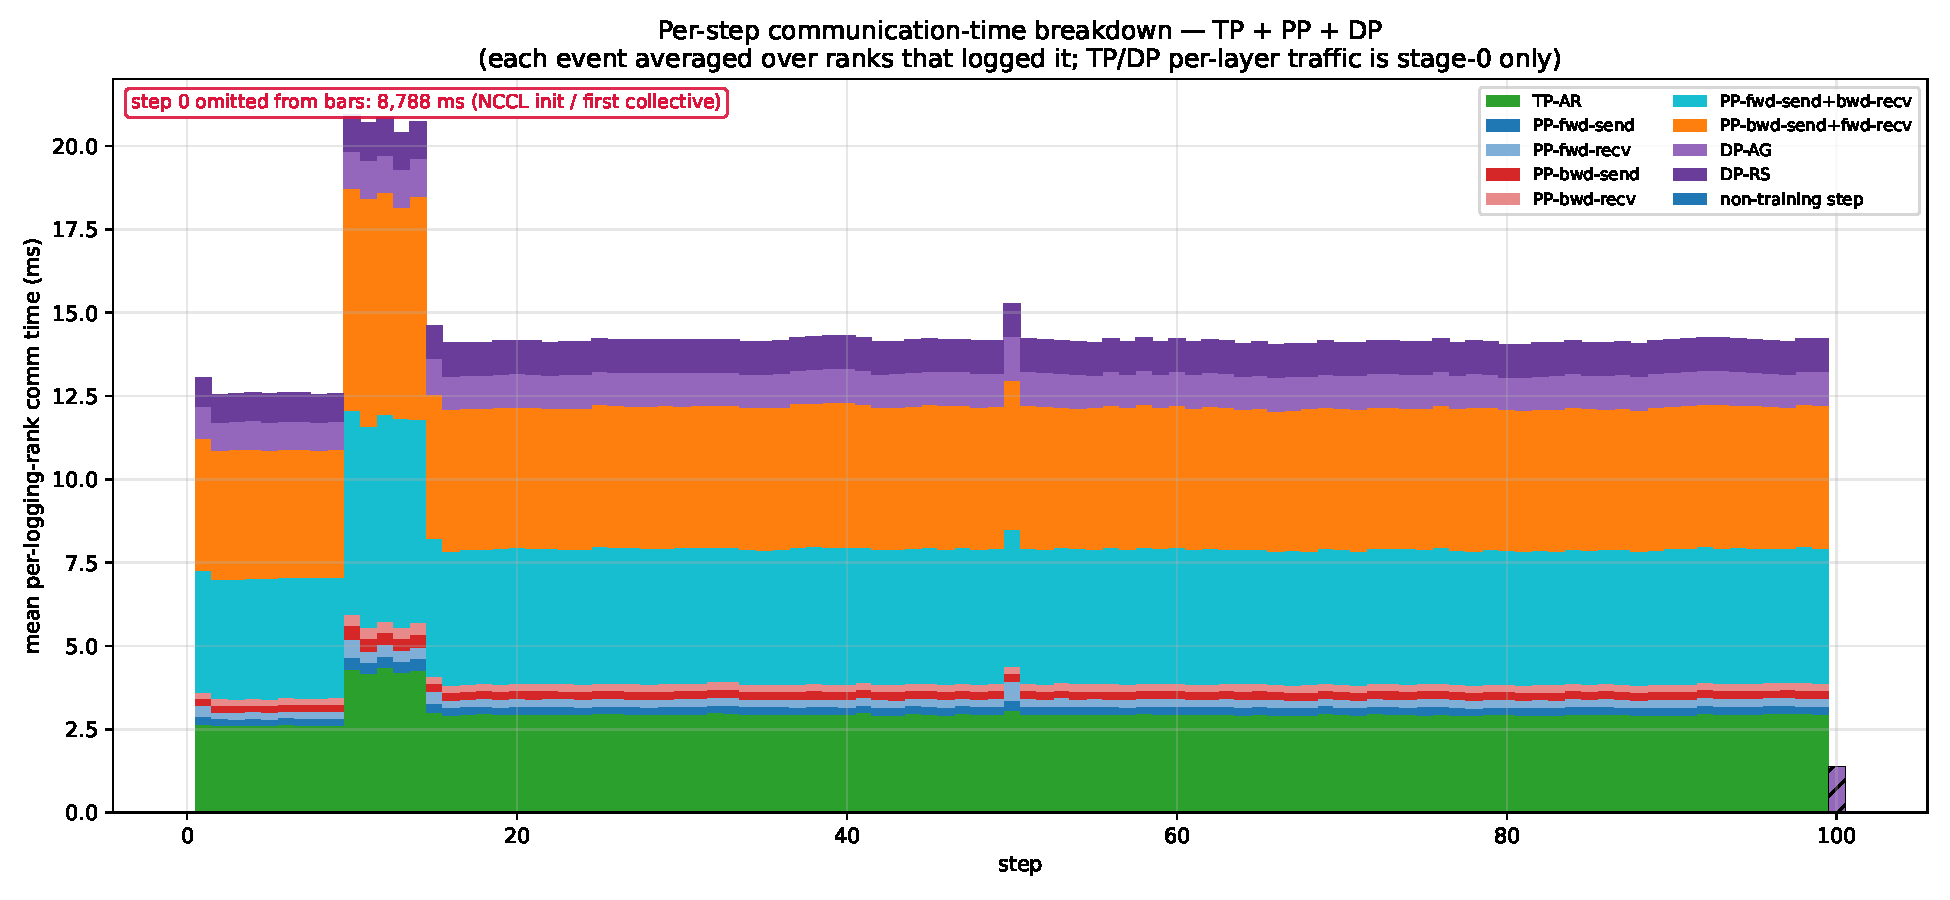
\includegraphics[width=\textwidth]{per_step_breakdown.pdf}
  \caption{Mean per-rank communication time per step, stacked by event.
    The fused pipeline exchange and TP all-reduce dominate the logged
    time; the asynchronous DP collectives barely register.}
  \label{fig:perstep}
\end{figure*}

\begin{figure*}[t]
  \centering
  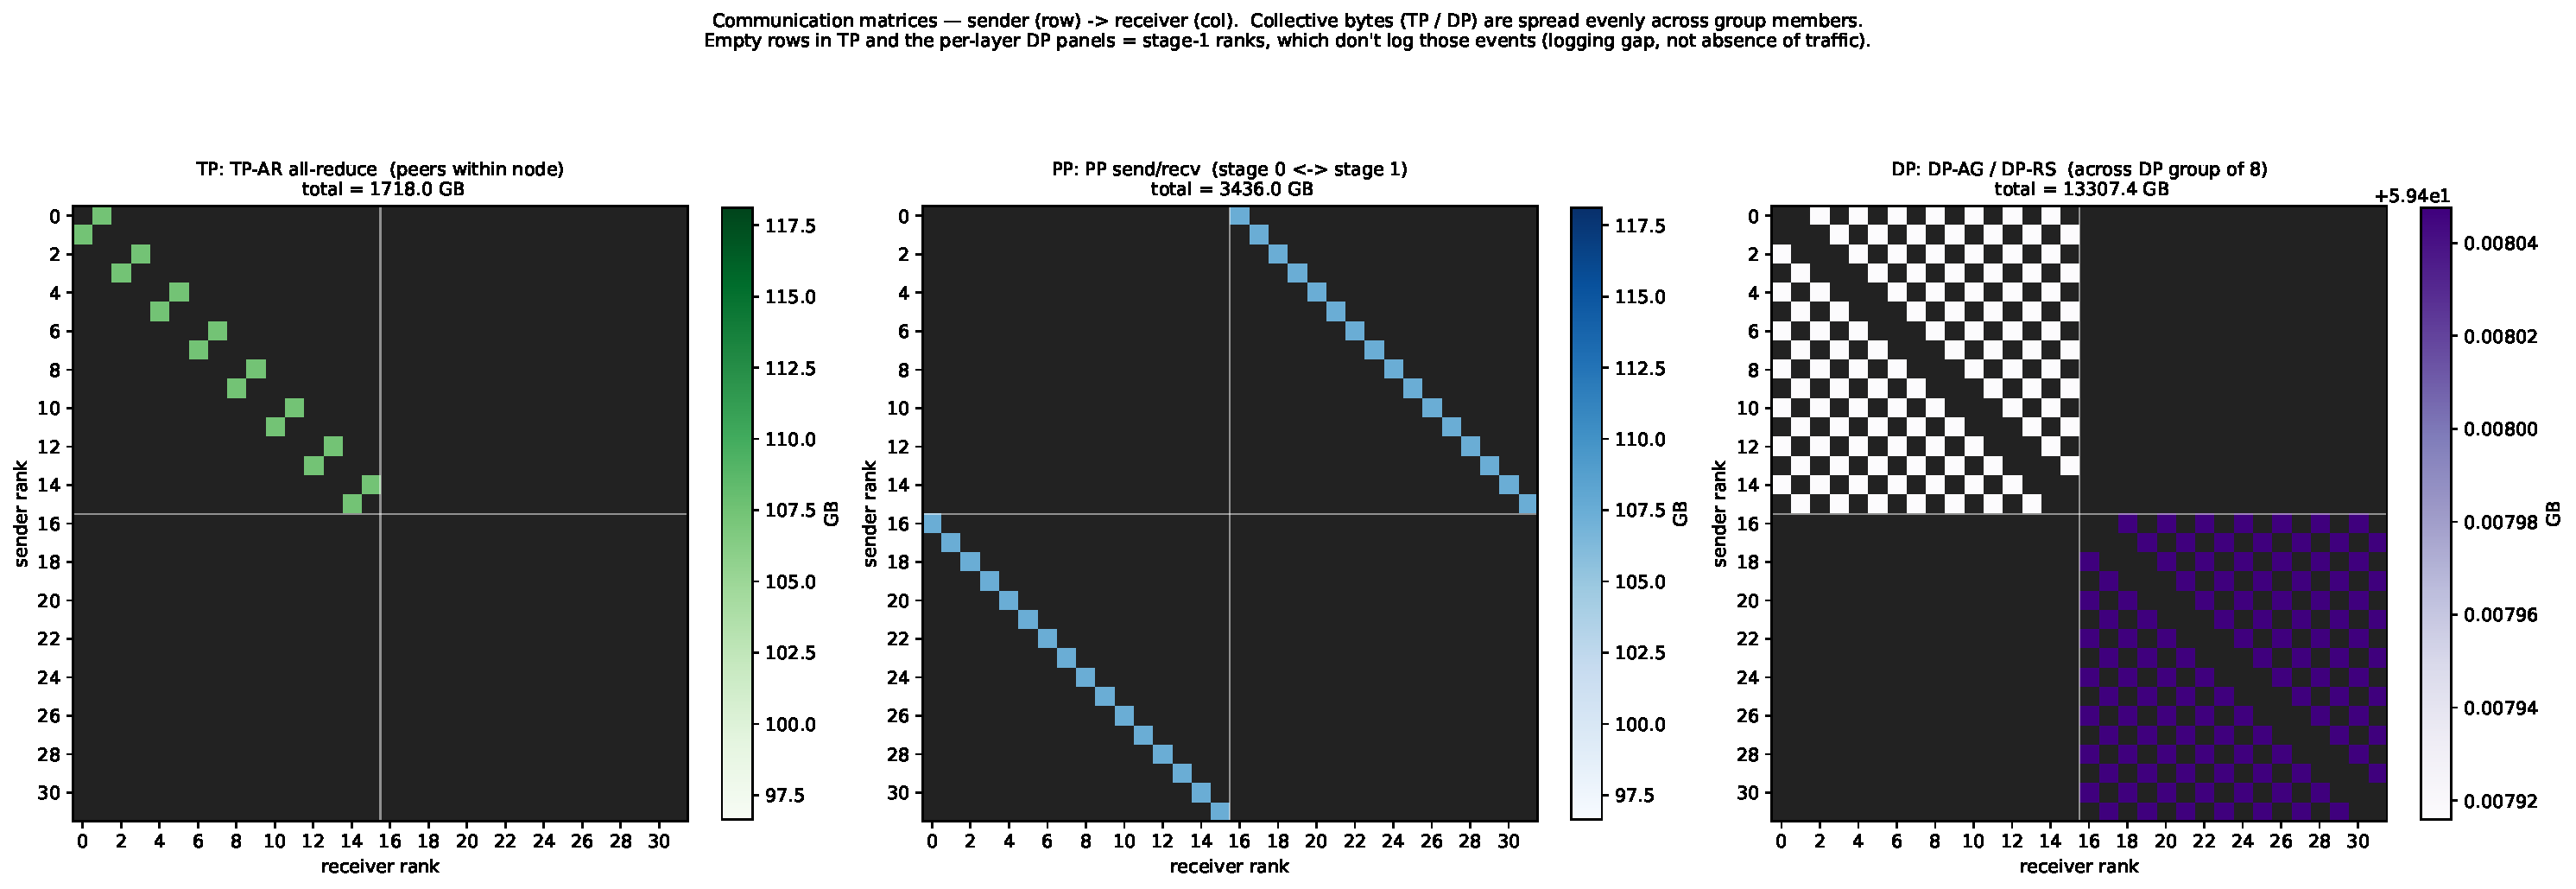
\includegraphics[width=\textwidth]{comm_matrix.pdf}
  \caption{Bytes sent, sender (row) $\to$ receiver (column), per group
    type. TP is intra-node, PP links the two stages, DP spreads across
    each 8-member group. Empty stage-1 rows are a logging gap.}
  \label{fig:commmatrix}
\end{figure*}

\begin{figure*}[t]
  \centering
  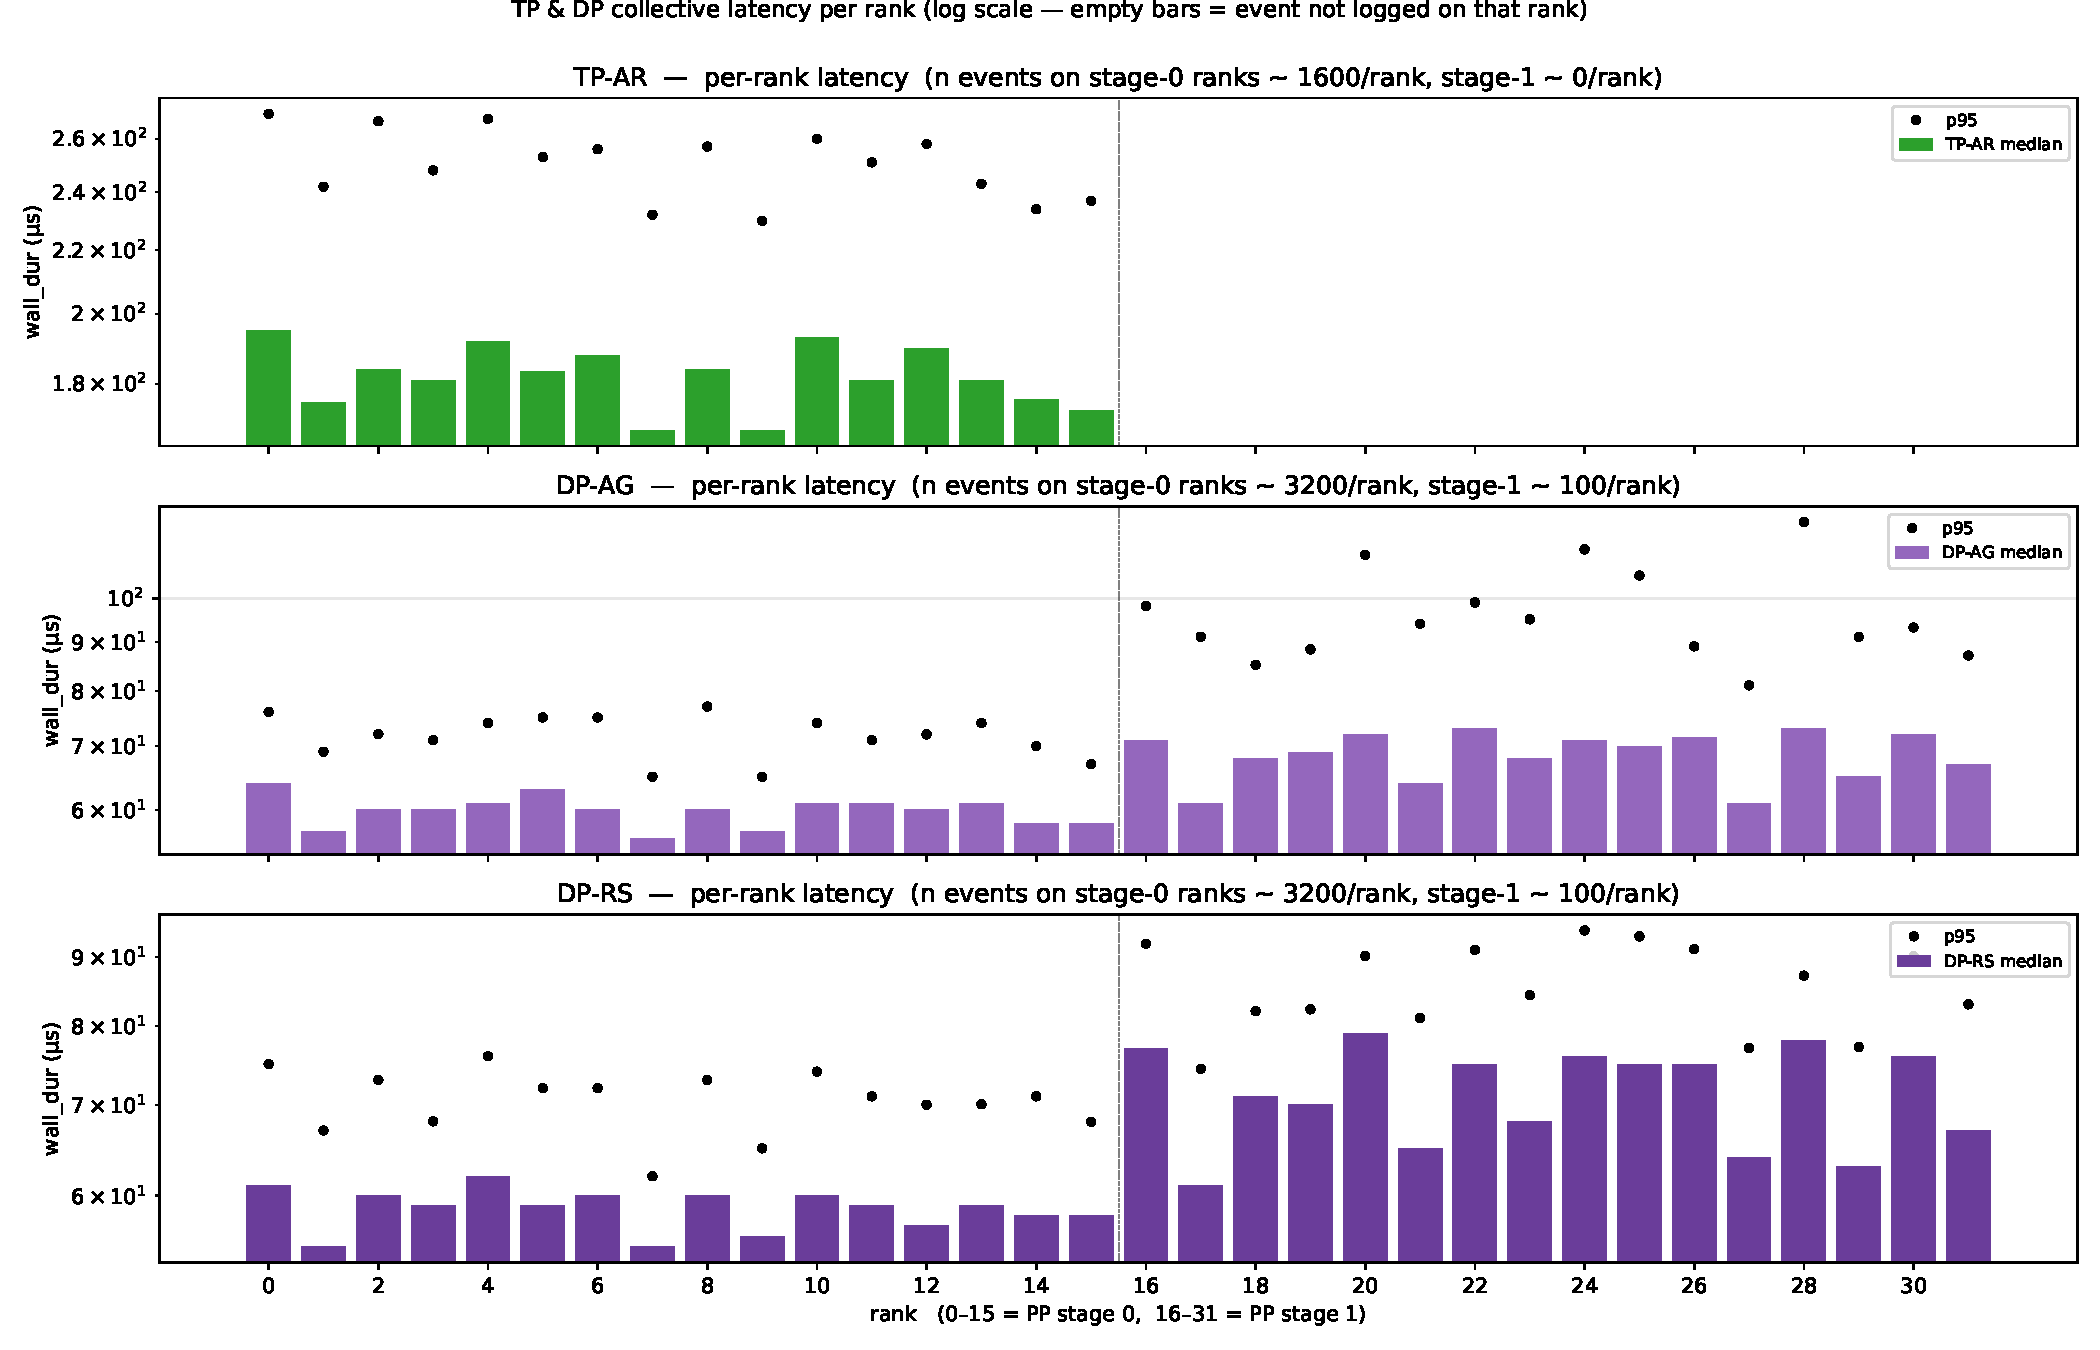
\includegraphics[width=\textwidth]{tp_dp_latency.pdf}
  \caption{Per-rank median/p95 latency for the TP and DP collectives
    (log scale). Latencies are uniform across ranks; empty bars mark
    events not logged on that stage.}
  \label{fig:tpdplat}
\end{figure*}

\begin{figure*}[t]
  \centering
  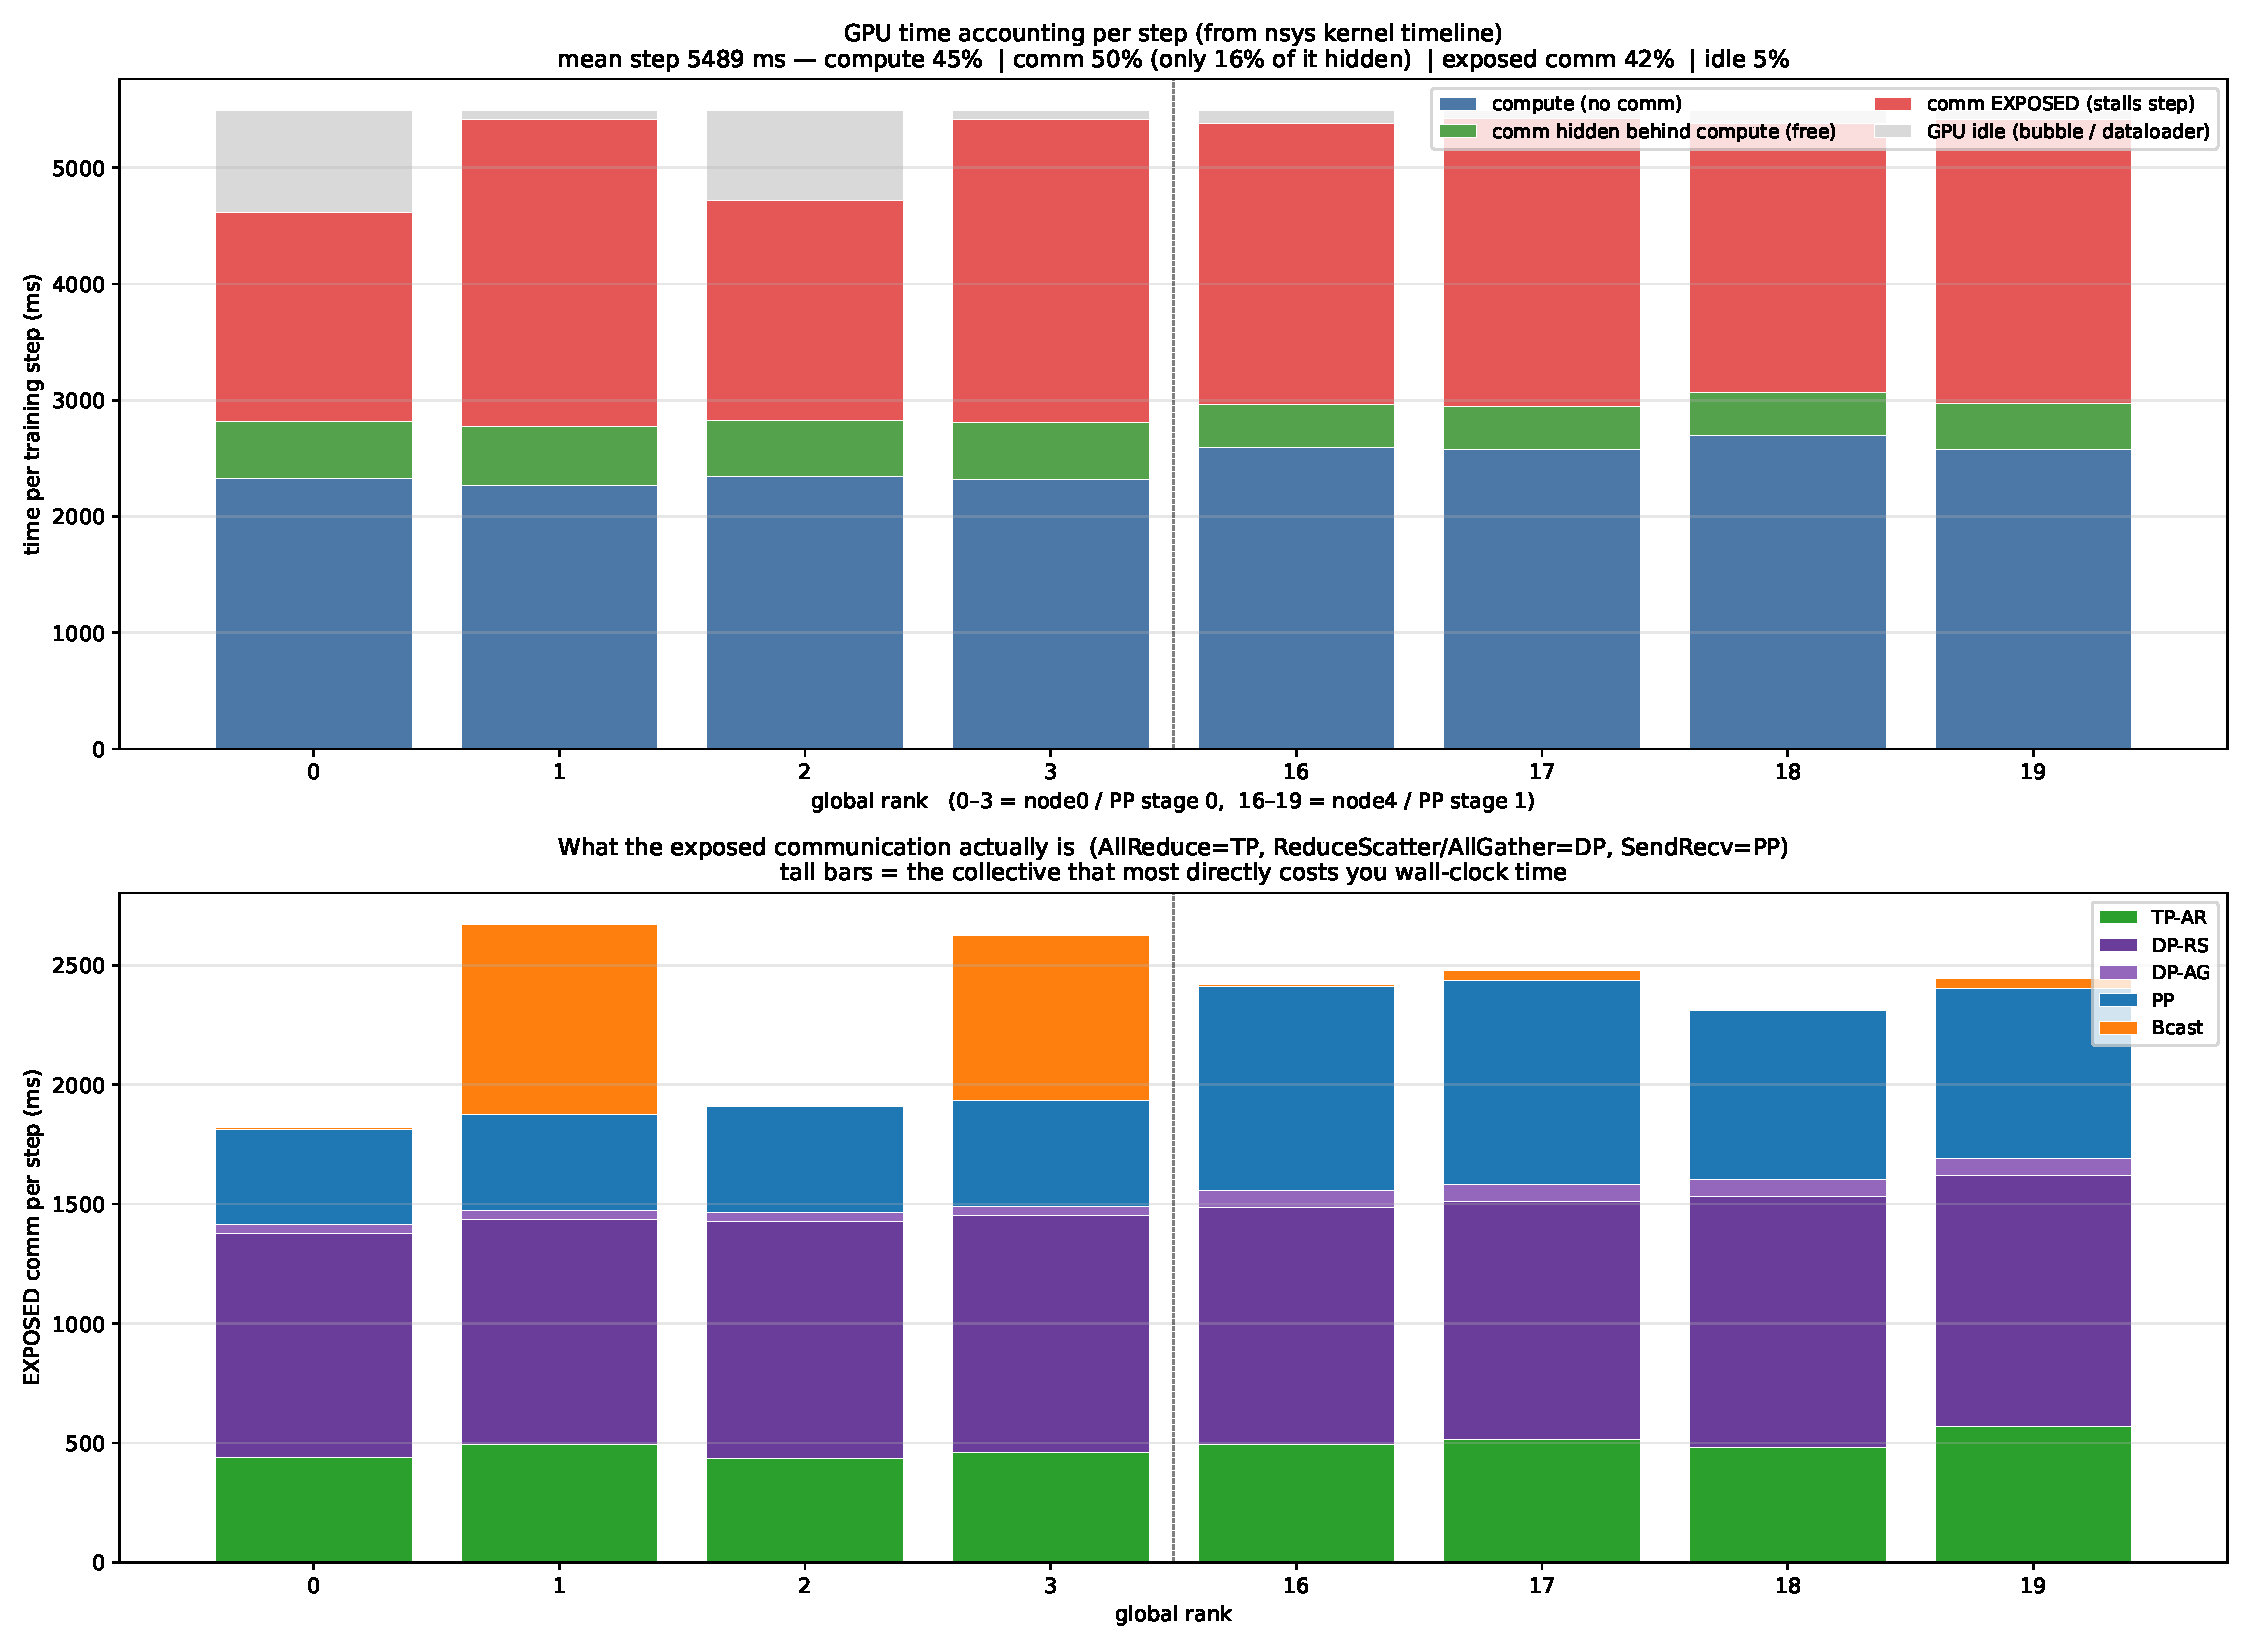
\includegraphics[width=\textwidth]{nsys_overlap_summary.pdf}
  \caption{Per-rank GPU-time accounting from the Nsight kernel timeline.
    \textbf{Top:} each step split into compute, communication hidden
    behind compute (free), \emph{exposed} communication (stalls the
    step), and GPU idle. \textbf{Bottom:} the exposed communication split
    by collective --- gradient reduce-scatter (purple) dominates; the
    input broadcast (orange) appears only on the TP-non-source ranks
    (1, 3, 17, 19).}
  \label{fig:overlap-summary}
\end{figure*}

\begin{figure*}[t]
  \centering
  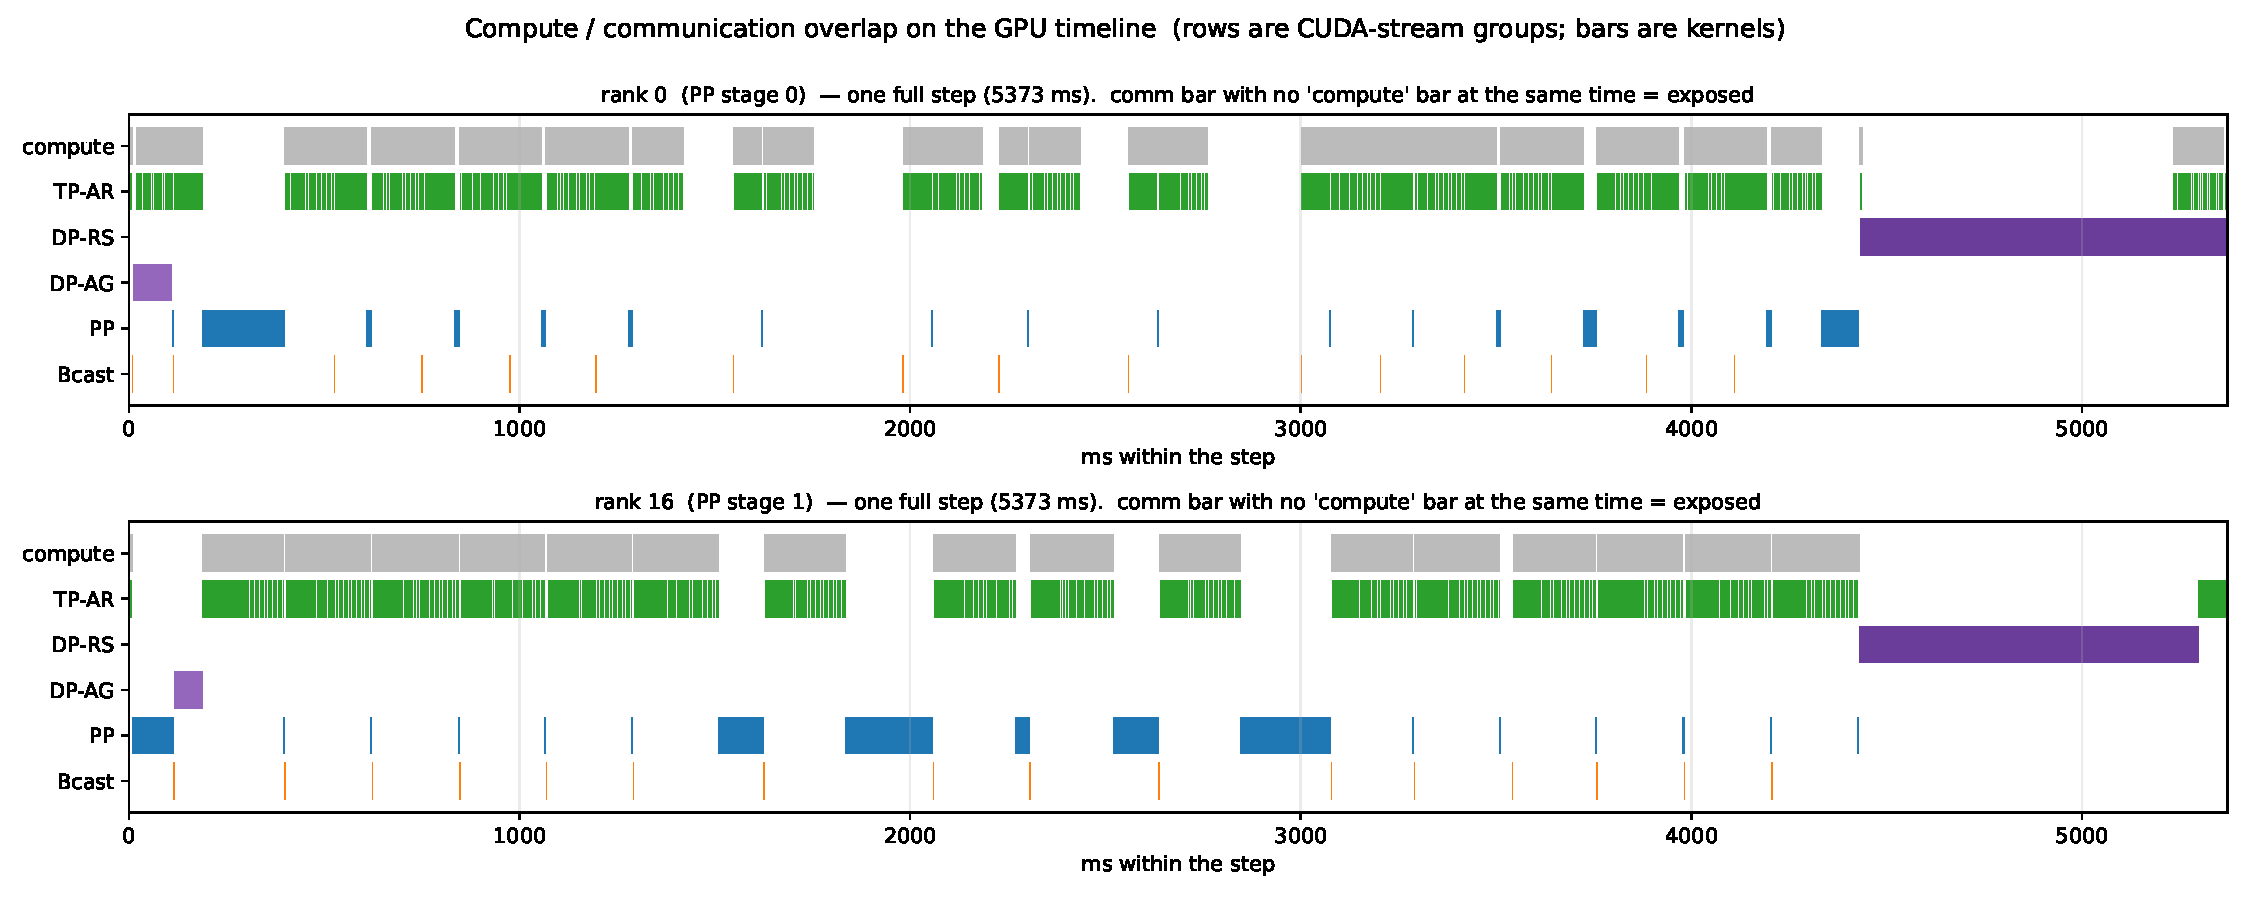
\includegraphics[width=\textwidth]{nsys_overlap_timeline.pdf}
  \caption{One full step on the GPU timeline for a stage-0 (top) and a
    stage-1 (bottom) rank; rows are CUDA-stream groups. Compute (grey)
    and TP all-reduce (green) overlap through forward/backward, but the
    DP reduce-scatter (purple) forms an exposed block at the end of the
    step with no compute above it --- the gradient sync that
    \texttt{--overlap-grad-reduce} fails to hide.}
  \label{fig:overlap-timeline}
\end{figure*}

\begin{figure}[t]
  \centering
  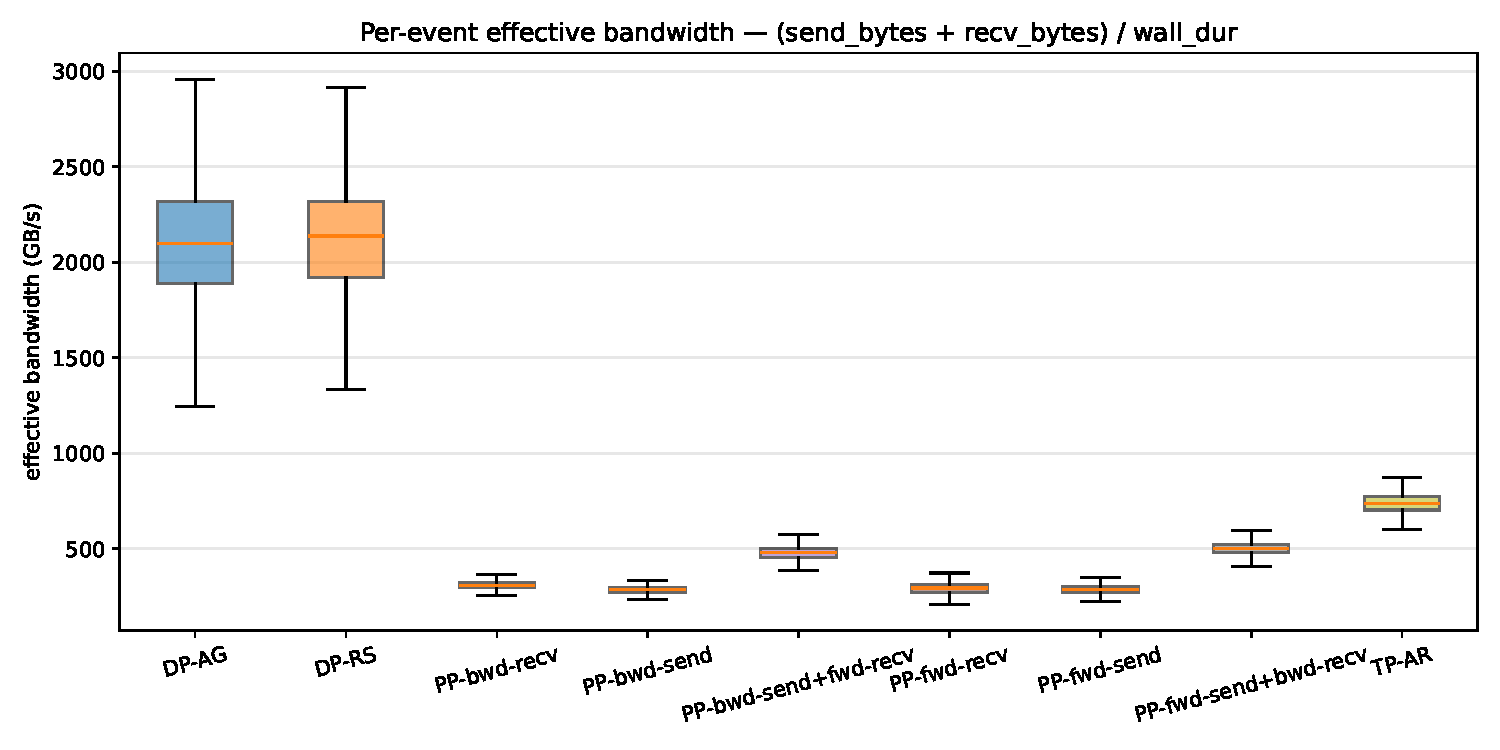
\includegraphics[width=\columnwidth]{bandwidth_distribution.pdf}
  \caption{Per-event effective bandwidth. Intra-node TP all-reduce
    (NVLink) far exceeds the inter-node PP/DP collectives (Slingshot).}
  \label{fig:bandwidth}
\end{figure}

\begin{figure}[t]
  \centering
  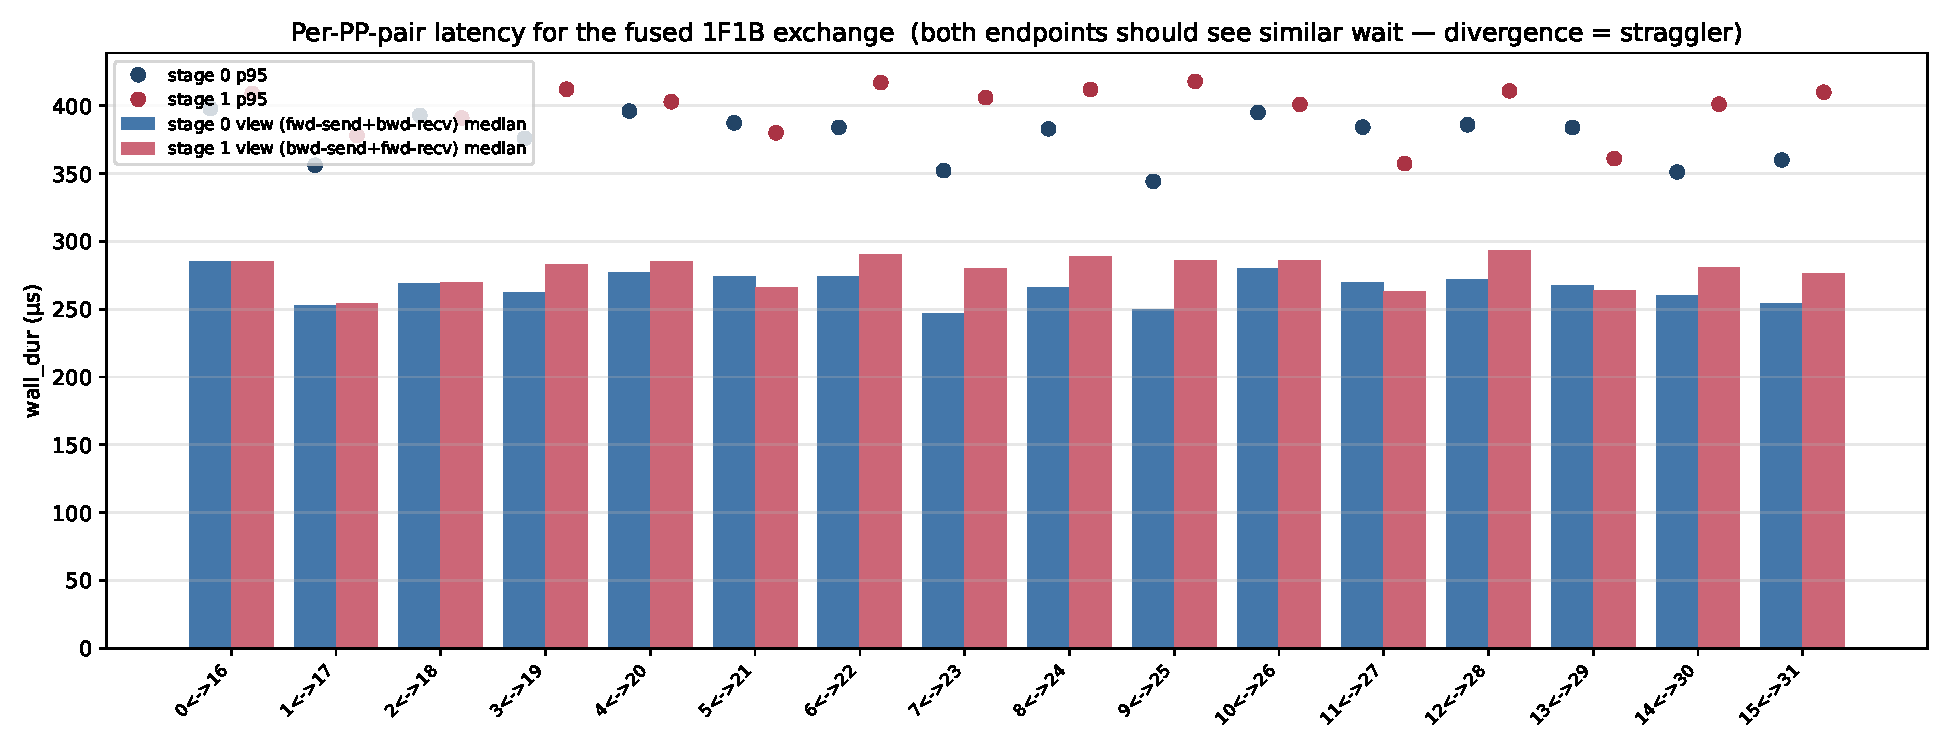
\includegraphics[width=\columnwidth]{pair_latency.pdf}
  \caption{Per-PP-pair latency of the fused 1F1B exchange. The two
    endpoints of each pair match, so the cost is structural, not a
    straggler.}
  \label{fig:pairlat}
\end{figure}

\begin{figure}[t]
  \centering
  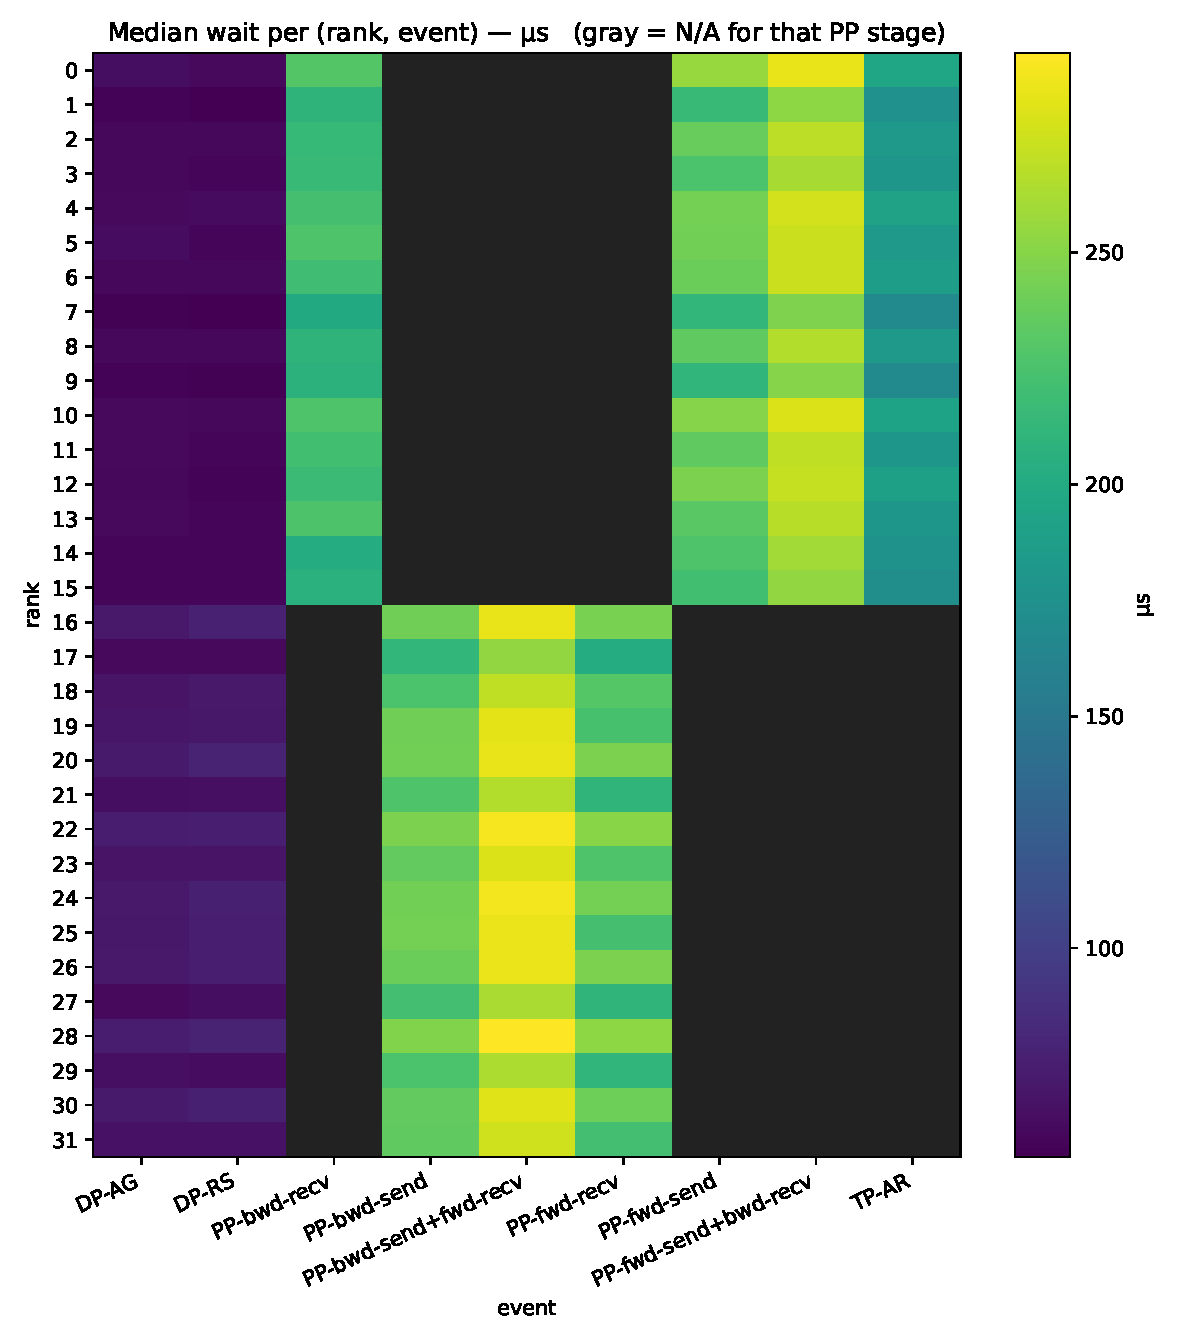
\includegraphics[width=\columnwidth]{rank_event_heatmap.pdf}
  \caption{Median wait per (rank, event). Grey cells mark events not
    logged on that PP stage.}
  \label{fig:heatmap}
\end{figure}
